Avec la création de la sous-offre \df, \tnp souhaitait compléter son offre de transformation numérique en proposant la fabrication de solutions technologiques en plus du conseil et de leur expertise métier.

Le projet bouclage de production s'inscrit dans cette stratégie. Le cabinet conseillait déjà des acteurs du secteur des mobilités, et il leur permet maintenant grâce à la \df d'également concevoir des solutions personnalisées lorsque leur besoin le nécessite.

\begin{figure}[H]
    \centering
    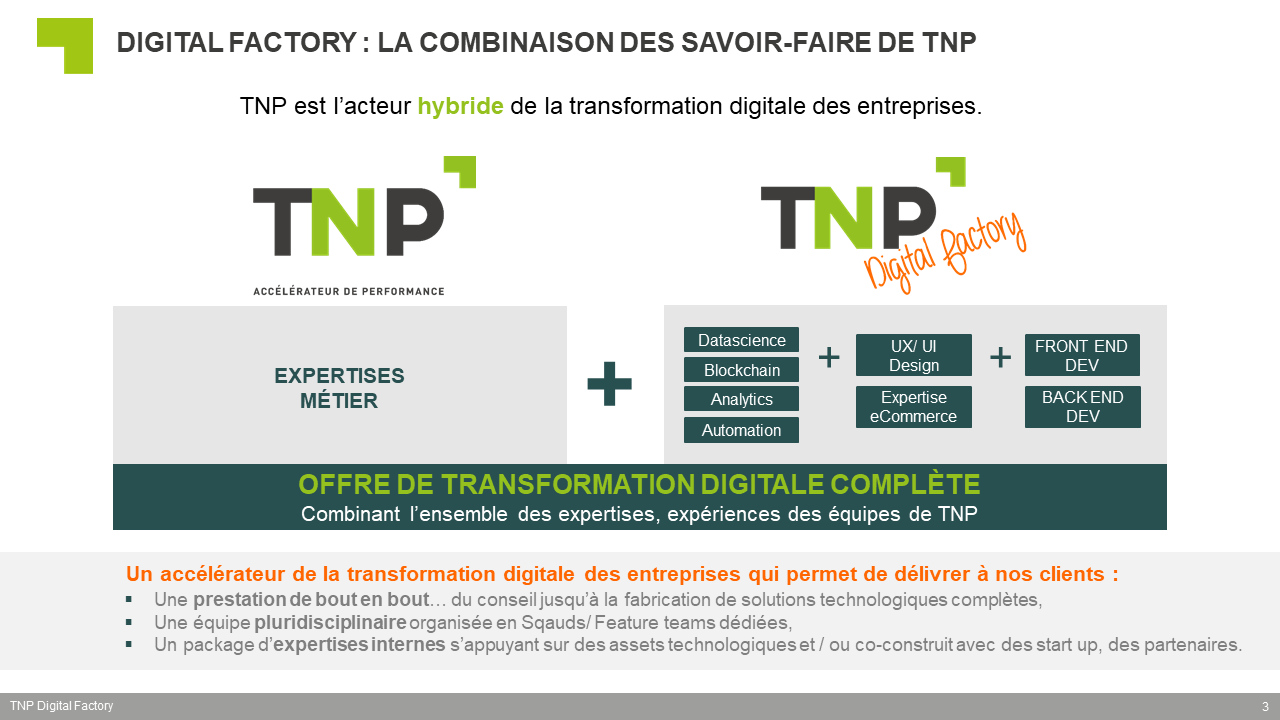
\includegraphics[width=1\linewidth]{img/offre_digital_factory_tnp.png}
    \caption{Intérêts de la Digital Factory pour \tnp}
\end{figure}

Les consultants du cabinet peuvent d'ores et déjà effectuer un travail de communication et publicité pour la \df. Cependant, celle-ci est encore jeune et peu connue même au sein du cabinet.

Il est donc dans l'intérêt de l'entreprise de faire connaître le service à ses consultants, notamment en réussissant des missions. Celles-ci permettront d'avoir un résultat concret pour mieux expliquer l'intérêt de la sous-offre aux consultants. Ces derniers deviendront par la suite des ambassadeurs de la \df chez leurs clients lorsque le besoin métier nécessitera une solution sur mesure conçue par \tnp.
